\section{Wyniki}

W tabeli \ref{table:results} przedstawiłem wyniki dla modeli z różnymi rozmiarami reprezentacji ukrytej oraz w różnych etapach nauki. Tak samo jak w poprzednich eksperymentach miarą pomiarową, którą obserwowałem było AUC na podstawie wartości funkcji straty. Można zauważyć szybkie przeuczenie się modeli, ponieważ w większości przypadków już od 3 epoki wyniki pogarszają się. Dodatkowo wraz z czasem pomiary stają się prawie jednakowe dla wszystkich rozmiarów. 

\begin{table}[h!]
	\centering
    \begin{tabular}{ l | c c c c c c }
 
    \multicolumn{1}{c}{Model} & \multicolumn{6}{c}{Epoka} \\
    \cmidrule(r){1-1} \cmidrule(r){2-7}
    %\toprule
     		& 1 & 2 & 3 & 20 & 60 & 80 \\ \cmidrule(r){2-7}
    VAE 20-d 	& 0.494 & 0.693 & 0.655 & 0.612 & 0.597 & 0.590 \\ \hline
    VAE 50-d 	& 0.552 & 0.686 & 0.697 & 0.616 & 0.606 & 0.592 \\ \hline
    VAE 100-d 	& 0.580 & 0.685 & \textbf{0.701} & 0.614 & 0.595 & 0.594 \\ \hline
    VAE 200-d   & 0.661 & 0.675 & 0.668 & 0.620 & 0.608 & 0.597 \\ \hline
    VAE 300-d   & 0.704 & 0.671 & 0.657 & 0.620 & 0.600 & 0.593 \\
    \toprule
    \end{tabular}
    \caption{AUC ze względu an rozmiar reprezentacji ukrytej i w różnych stadiach nauki}
	\label{table:results}
\end{table}

\section{Analiza}

Zajmę się analizą modelu, który osiągnął najlepszy rezultat, czyli autoenkodera wariacyjnego bazującego na reprezentacji ukrytej rozmiaru 100 po 3 epokach nauki. Na rysunku \ref{fig:soft_vae} widać wykres z zaznaczonymi poszczególnymi składnikami kosztu, czyli koszt KLD i rekonstrukcji NLL. Przypomnę, że na bazie ich sumy liczona jest krzywa ROC. Można zauważyć specyficzny rozkład punktów. Ponadto na rysunku pokazane są przykładowe rekonstrukcje, ale prawdopodobnie ze względu na zbyt krótki czas nauki nie prezentują się one najlepiej.

\begin{figure}[h!]
    \centering
    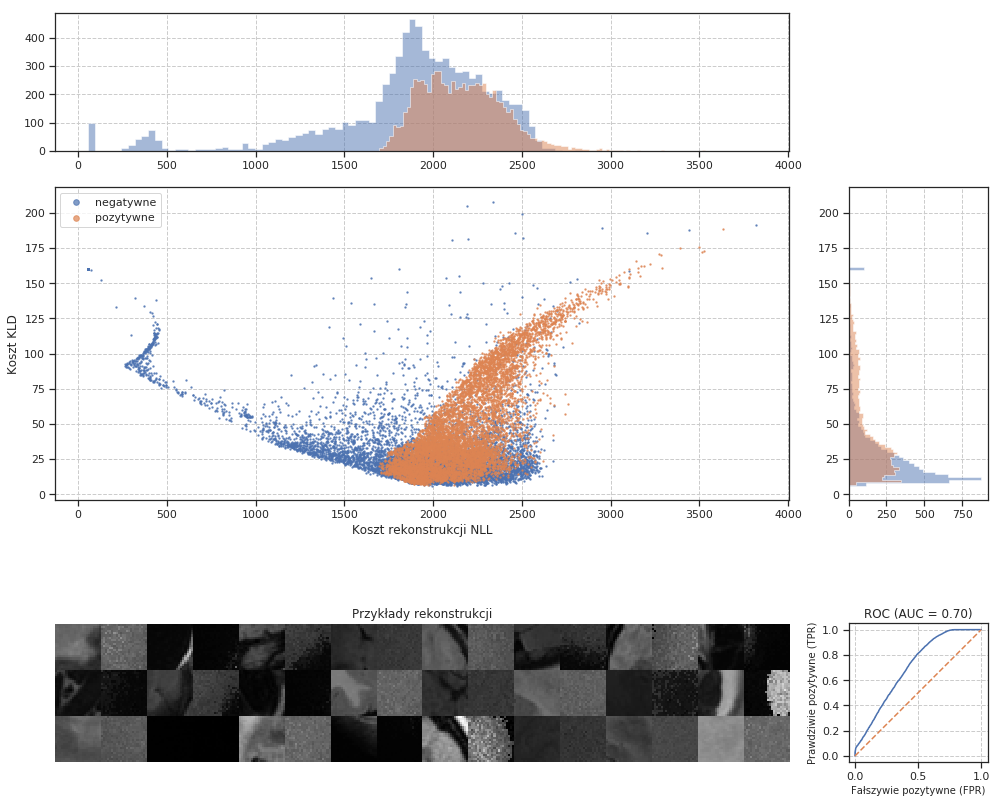
\includegraphics[width=1.0\textwidth]{images/soft_vae_v2}
    \caption{Poszczególne składniki kosztu dla modelu z najlepszą separowalnością}
    \label{fig:soft_vae}
\end{figure}

Chciałbym w tym miejscu wrócić to dwóch grup punktów, które się dobrze separowały i sprawdzić jaka ich własność mogła na to wpłynąć. Prostą obserwacją z poprzedniej analizy danych jest to, że obrazki dotyczące komórek nowotworowych są z reguły jaśniejsze od tych dotyczących zdrowych. Jasność obrazka będę utożsamiał z sumą pikseli. Niska wartość będzie oznaczać dla mnie ciemne obrazki, a wysoka jasne. Na wykresie \ref{fig:pixels_hist} znajduje się histogram dla sumy piksli zdjęć z zestawu testowego.

\begin{figure}[h!]
    \centering
    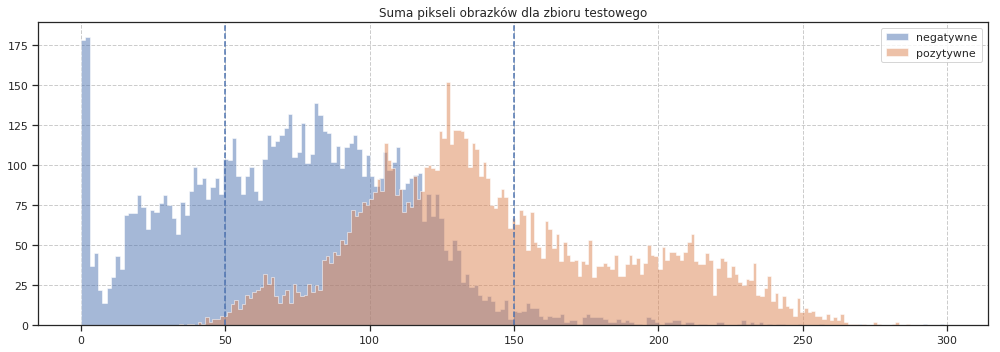
\includegraphics[width=1.0\textwidth]{images/pixels_hist_v2}
    \caption{Rozkład sum pikseli dla obrazków ze zbioru testowego}
    \label{fig:pixels_hist}
\end{figure}

Można zauważyć, że występują dwa progi, które w łatwy sposób klasyfikują sporą część danych z dużą dokładnością. Jest to odpowiednio 50.0 dla obrazków negatywnych i 150.0 dla pozytywnych. Znalazłem obrazki, które można zidentyfikować w ten sposób i zaznaczyłem ich położenie na oryginalnym wykresie. W ten sposób otrzymałem wykres \ref{fig:soft_vae_th}.

\begin{figure}[h!]
    \centering
    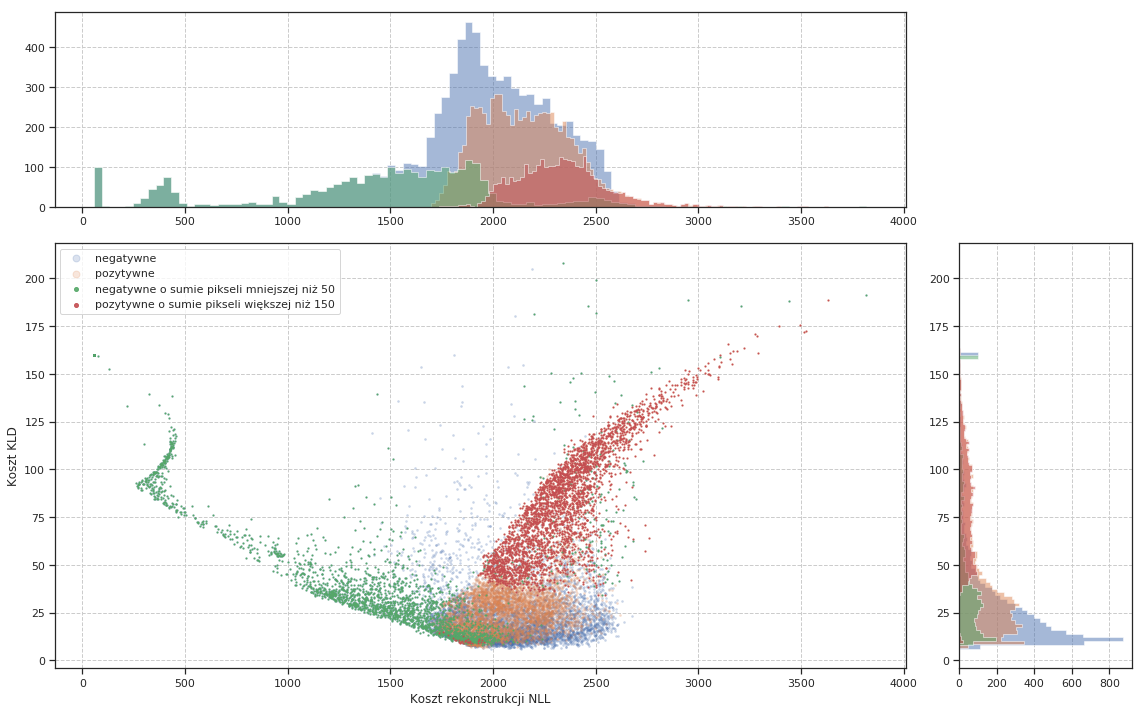
\includegraphics[width=1.0\textwidth]{images/soft_vae_th_v2}
    \caption{Zaznaczenie obrazków o konkretnych sumach pikseli}
    \label{fig:soft_vae_th}
\end{figure}

Widać, że są to dokładnie te same grupy danych, które dobrze się separowały. Wniosek z tego jest taki, że w wypadku modelu uczonego prawie jedynie na obrazkach bez zmian nowotworowych, ciemne próbki są bardzo prawdopodobne, a jasne już nie. Model nie dał rady znaleźć innych cech, na podstawie których można byłoby rozróżniać te dwie grupy.





